\documentclass[11pt]{article}

\usepackage{fullpage}
\usepackage{amsfonts}
\usepackage{graphicx}

\def\eq1{y=\frac{x}{3x^2+x+1}}
\def\labelaxes{Remeber to include a scale and label your axes.}

\begin{document}

The set of Natural numbers is denoted by $\mathbb{N}$.

The set of Natural numbers is denoted by $\mathbb{Z}$.

The set of Real nembers if denoted by $\ mathbb{R}$

Graph $\eq1$. \labelaxes

\begin{center}
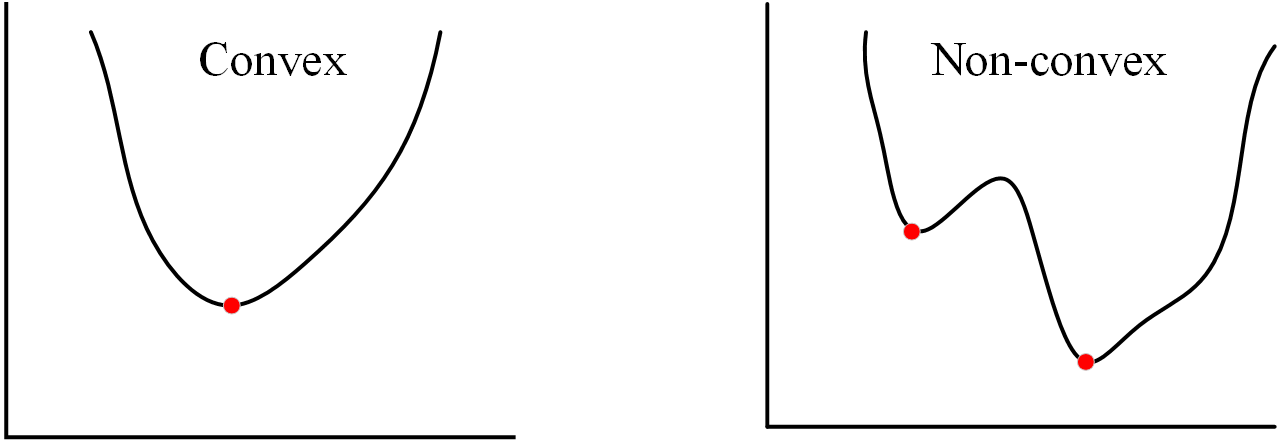
\includegraphics[scale=0.5]{Nonconvex1.png}
\end{center}

% When we include the images, the image and latex file have to be at the same folder


Image 
Identify the asymptotes for the graph of $\eq1$

\end{document}